\let\negmedspace\undefined
\let\negthickspace\undefined
\documentclass[journal]{IEEEtran}
\usepackage[a5paper, margin=10mm, onecolumn]{geometry}
\usepackage{tfrupee} 

\setlength{\headheight}{1cm} 
\setlength{\headsep}{0mm}  
\usepackage{gvv-book}
\usepackage{gvv}
\usepackage{cite}
\usepackage{amsmath,amssymb,amsfonts,amsthm}
\usepackage{algorithmic}
\usepackage{graphicx}
\usepackage{textcomp}
\usepackage{xcolor}
\usepackage{txfonts}
\usepackage{listings}
\usepackage{enumitem}
\usepackage{mathtools}
\usepackage{gensymb}
\usepackage{comment}
\usepackage[breaklinks=true]{hyperref}
\usepackage{tkz-euclide} 
\usepackage{listings}
% \usepackage{gvv}                                        
\def\inputGnumericTable{}                                 
\usepackage[latin1]{inputenc}                                
\usepackage{color}                                            
\usepackage{array}                                            
\usepackage{longtable}                                       
\usepackage{calc}                                             
\usepackage{multirow}                                         
\usepackage{hhline}                                           
\usepackage{ifthen}                                           
\usepackage{lscape}
\usepackage{tikz}
\usetikzlibrary{patterns}
\begin{document}

\bibliographystyle{IEEEtran}
\vspace{3cm}


\title{GATE 2025 ME }
\author{ee25btech11029- Jnanesh Sathisha Karmar}
\maketitle
% \maketitle
% \newpage
% \bigskip
{\let\newpage\relax\maketitle}

\renewcommand{\thefigure}{\theenumi}
\renewcommand{\thetable}{\theenumi}
\setlength{\intextsep}{10pt} % Space between text and floats
\begin{enumerate}[leftmargin=0pt]

\item
$Fish\colon Shoal\colon\colon Lion\colon\underline{\hspace{2cm}}$
\vspace{0.2cm}
\begin{enumerate}
\begin{multicols}{4}
\item Pride
\item School
\item Forest
\item Series
\end{multicols}
\end{enumerate}
\hfill{\brak{\text{GATE ME 2025}}}

\item
Identify the grammatically correct sentence$\colon$
\vspace{0.2cm}
\begin{enumerate}
\begin{multicols}{2}
\item It is I who am responsible for this fiasco.
\item It is myself who is responsible for this fiasco.

\item It is I who is responsible for this fiasco.

\item It is I who are responsible for this fiasco.
\end{multicols}
\end{enumerate}
\hfill{\brak{\text{GATE ME 2025}}}

\item
Two cars, P and Q, start from a point X in India at $10$ AM. Car P travels North with a speed of $25\,\text{km/h}$ and car Q travels East with a speed of $30\,\text{km/h}$. Car P travels continuously but car Q stops for some time after travelling for one hour. If both the cars are at the same distance from X at $11\colon30$ AM, for how long \brak{\text{in minutes}} did car Q stop?

\vspace{0.2cm}
\begin{enumerate}
\begin{multicols}{4}
\item $10$
\item $12$
\item $15$
\item $18$
\end{multicols}
\end{enumerate}
\hfill{\brak{\text{GATE ME 2025}}}

\item
The ceiling function of a real number $x$, denoted by $ce\brak{x}$, is defined as the smallest integer that is greater than or equal to $x$. Similarly, the floor function, denoted by $fl\brak{x}$, is defined as the largest integer that is smaller than or equal to $x$. Which one of the following statements is NOT correct for all possible values of $x$?

\vspace{0.2cm}
\begin{enumerate}
\begin{multicols}{2}
\item $ce\brak{x} \geq x$
\item $fl\brak{x} \leq x$
\item $ce\brak{x}\geq fl\brak{x}$
\item $fl\brak{x}<ce\brak{x}$
\end{multicols}
\end{enumerate}
\hfill{\brak{\text{GATE ME 2025}}}

\item
P and Q play chess frequently against each other. Of these matches, P has won $80\%$ of the matches, drawn $15\%$ and lost $5\%$. If they play $3$ more matches, what is the probability of P winning exactly $2$ of these $3$ matches?

\vspace{0.2cm}
\begin{enumerate}
\begin{multicols}{2}
\item $\dfrac{48}{125}$
\item $\dfrac{16}{125}$
\item $\dfrac{16}{25}$
\item $\dfrac{25}{48}$
\end{multicols}
\end{enumerate}
\hfill{\brak{\text{GATE ME 2025}}}

\item
Identify the option that has the most appropriate sequence such that a coherent paragraph is formed$\colon$\\
P.\ At once, without thinking much, people rushed towards the city in hordes with the sole aim of grabbing as much gold as they could.\\
Q.\ However, little did they realize about the impending hardships they would have to face on their way to the city$\colon$ miles of mud, unfriendly forests, hungry beasts and inimical local lords -- all of which would reduce their chances of getting gold to almost zero.\\
R.\ All of them thought that easily they could lay their hands on gold and become wealthy overnight.\\
S.\ About a hundred years ago, the news that gold had been discovered in Kolar spread like wildfire and the whole State was in raptures.

\vspace{0.2cm}
\begin{enumerate}
\begin{multicols}{2}
\item P$\to$Q$\to$R$\to$S
\item S$\to$Q$\to$P$\to$R
\item Q$\to$S$\to$R$\to$P
\item S$\to$R$\to$Q$\to$P
\end{multicols}
\end{enumerate}
\hfill{\brak{\text{GATE ME 2025}}}

\item
If HIDE and CAGE are coded as $19$-$23$-$7$-$11$ and $5$-$2$-$17$-$11$ respectively, then what is the code for HIGH?

\vspace{0.2cm}
\begin{enumerate}
\begin{multicols}{2}
\item $5$-$17$-$1$-$2$
\item $17$-$19$-$13$-$17$
\item $13$-$3$-$1$-$2$
\item $19$-$23$-$17$-$19$
\end{multicols}
\end{enumerate}
\hfill{\brak{\text{GATE ME 2025}}}

\item
The given figure is reflected about the horizontal dashed line and then rotated clockwise by $90\degree$ about an axis perpendicular to the plane of the figure. Which one of the following options correctly shows the resultant figure?
\begin{figure}[H]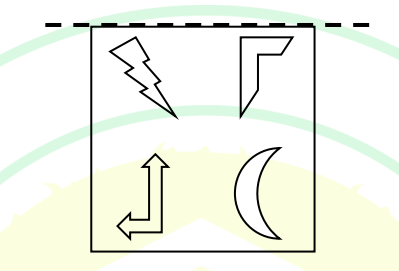
\includegraphics[width=0.5\columnwidth]{Figs/image (89).png}\caption*{}\label{fig:q8}\end{figure}
\vspace{0.2cm}
\begin{enumerate}
\begin{multicols}{2}
\item \begin{figure}[H]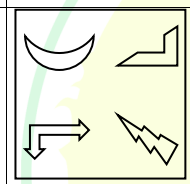
\includegraphics[width=0.5\columnwidth]{Figs/image (90).png}\caption*{}\label{fig:a}\end{figure}
\item \begin{figure}[H]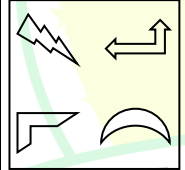
\includegraphics[width=0.5\columnwidth]{Figs/image (91).png}\caption*{}\label{fig:q8b}\end{figure}


\item
\begin{figure}[H]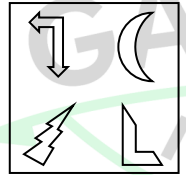
\includegraphics[width=0.5\columnwidth]{Figs/image (93).png}\caption*{}\label{fig:q8c}\end{figure}
\item 
\begin{figure}[H]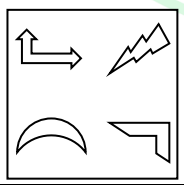
\includegraphics[width=0.5\columnwidth]{Figs/image (94).png}\caption*{}\label{fig:q8d}\end{figure}

\end{multicols}
\end{enumerate}
\hfill{\brak{\text{GATE ME 2025}}}

\item
Which one of the following options has the correct sequence of objects arranged in the increasing number of mirror lines \brak{\text{lines of symmetry}}?

\vspace{0.2cm}
\begin{enumerate}
\begin{multicols}{2}
\item Circle; Square; Equilateral triangle; Isosceles triangle
\item Isosceles triangle; Equilateral triangle; Square; Circle
\item Equilateral triangle; Isosceles triangle; Square; Circle
\item Isosceles triangle; Square; Equilateral triangle; Circle
\end{multicols}
\end{enumerate}
\hfill{\brak{\text{GATE ME 2025}}}

\item
A final year student appears for placement interview in two companies, S and T. Based on her interview performance, she estimates the probability of receiving job offers from companies S and T to be $0.8$ and $0.6$, respectively. Let $p$ be the probability that she receives job offers from both the companies. Select the most appropriate option.

\vspace{0.2cm}
\begin{enumerate}
\begin{multicols}{2}
\item $0$
\item $0.4\leq p\leq 0.6$
\item $0.2\leq p\leq 0.4$
\item $0.6\leq p\leq 1.0$
\end{multicols}
\end{enumerate}
\hfill{\brak{\text{GATE ME 2025}}}


\item
Let $A$ and $B$ be real symmetric matrices of same size. Which one of the following options is correct?

\vspace{0.2cm}
\begin{enumerate}
\begin{multicols}{2}
\item $A^T = A^{-1}$
\item $AB = BA$
\item $(AB)^T = B^T A^T$
\item $A = A^{-1}$
\end{multicols}
\end{enumerate}
\hfill{\brak{\text{GATE ME 2025}}}

\item
For the differential equation given below, which one of the following options is correct?\\
$\dfrac{\partial^2 u}{\partial x^2} + \dfrac{\partial^2 u}{\partial y^2} = 0$  for $0 \leq x \leq 1,\, 0 \leq y \leq 1$
\vspace{0.2cm}
\begin{enumerate}
\begin{multicols}{2}
\item $u = e^{x+y}$ is a solution for all $x$ and $y$
\item $u = -e^x \sin x \sin y$ is a solution for all $x$ and $y$
\item $u = \sin x \sin y$ is a solution for all $x$ and $y$
\item $u = \cos x$ is a solution for all $x$ and $y$
\end{multicols}
\end{enumerate}
\hfill{\brak{\text{GATE ME 2025}}}

\item
The divergence of the curl of a vector field is

\vspace{0.2cm}
\begin{enumerate}
\begin{multicols}{2}
\item the magnitude of this vector field
\item the argument of this vector field
\item the magnitude of the curl of this vector field
\item zero
\end{multicols}
\end{enumerate}
\hfill{\brak{\text{GATE ME 2025}}}

\item
If two unbiased coins are tossed, then what is the probability of having at least one head?

\vspace{0.2cm}
\begin{enumerate}
\begin{multicols}{2}
\item $0.25$
\item $0.5$
\item $0.75$
\item $1$
\end{multicols}
\end{enumerate}
\hfill{\brak{\text{GATE ME 2025}}}

\item
Let a spherical block of ice at $-7\,\degree C$ be exposed to atmospheric air at $30\,\degree C$ with the gravitational direction as shown in the figure below. What will be the overall direction of air flow in this situation?
\begin{figure}[H]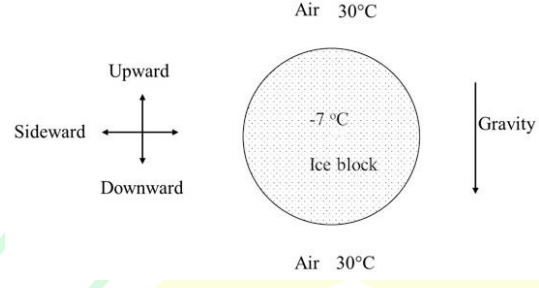
\includegraphics[width=0.5\columnwidth]{Figs/image (95).png}\caption*{}\label{fig:q15}\end{figure}

\vspace{0.2cm}
\begin{enumerate}
\begin{multicols}{2}
\item Upward
\item Downward
\item NO motion
\item Sideward
\end{multicols}
\end{enumerate}
\hfill{\brak{\text{GATE ME 2025}}}

\item
Consider two identical tanks with a bottom hole of diameter $d$. One tank is filled with water and the other tank is filled with engine oil. The height of the fluid column $h$ is same in both the cases. The fluid exit velocity in the two tanks are $V_1$ and $V_2$. Neglecting all losses, which one of the following options is correct?
\begin{figure}[H]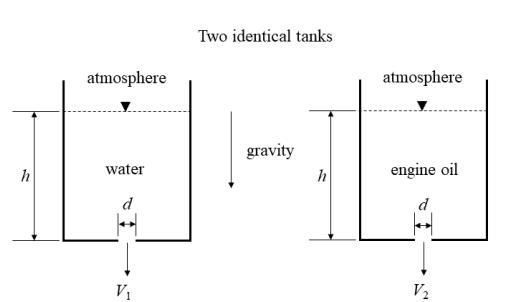
\includegraphics[width=0.5\columnwidth]{Figs/image (96).png}\caption*{}\label{fig:q16}\end{figure}
\vspace{0.2cm}
\begin{enumerate}
\begin{multicols}{2}
\item $V_2 > V_1$
\item $V_2 = V_1$
\item $V_2 < V_1$
\item Insufficient data to definitively conclude the relationship between $V_1$ and $V_2$
\end{multicols}
\end{enumerate}
\hfill{\brak{\text{GATE ME 2025}}}

\item
In a laboratory experiment using a scaled down model to measure scour at a bridge pier, the Froude number is important. The ratio of the prototype length to the model length is $100$. If the velocity of the model is $1\,\text{m/s}$, the velocity \brak{\text{in m/s}} of the prototype is

\vspace{0.2cm}
\begin{enumerate}
\begin{multicols}{2}
\item $0.1$
\item $1$
\item $10$
\item $100$
\end{multicols}
\end{enumerate}
\hfill{\brak{\text{GATE ME 2025}}}

\item
Air inside a rigid, thermally-insulated tank undergoes stirring as shown in the figure below. Which one of the following options is correct?
\begin{figure}[H]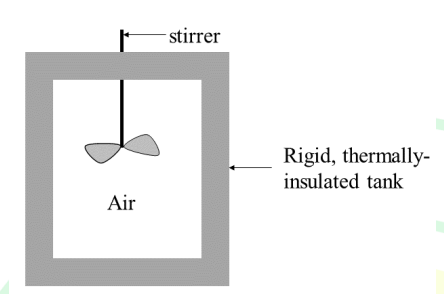
\includegraphics[width=0.5\columnwidth]{Figs/image (97).png}\caption*{}\label{fig:q18}\end{figure}
\vspace{0.2cm}
\begin{enumerate}
\begin{multicols}{2}
\item The enthalpy of the air increases while the entropy of the air remains constant
\item Both the enthalpy and the entropy of the air remain constant
\item Both the enthalpy and the entropy of the air increase
\item The enthalpy of the air decreases while the entropy of the air increases
\end{multicols}
\end{enumerate}
\hfill{\brak{\text{GATE ME 2025}}}

\item
In a psychrometric chart, one axis represents dry-bulb temperature. The axis, that is perpendicular to the dry-bulb temperature axis, represents

\vspace{0.2cm}
\begin{enumerate}
\begin{multicols}{2}
\item wet-bulb temperature
\item specific humidity
\item relative humidity
\item enthalpy
\end{multicols}
\end{enumerate}
\hfill{\brak{\text{GATE ME 2025}}}

\item
Among the following surface hardening processes, steel is heated to the lowest temperature in

\vspace{0.2cm}
\begin{enumerate}
\begin{multicols}{2}
\item carburizing
\item cyaniding
\item nitriding
\item carbonitriding
\end{multicols}
\end{enumerate}
\hfill{\brak{\text{GATE ME 2025}}}

\item
The welding process commonly used for fabricating tailor-welded blanks of dissimilar thickness for automotive applications is

\vspace{0.2cm}
\begin{enumerate}
\begin{multicols}{2}
\item gas welding
\item laser welding
\item arc welding
\item friction welding
\end{multicols}
\end{enumerate}
\hfill{\brak{\text{GATE ME 2025}}}

\item
The yield stress of a metal in uniaxial tension is $200\,\text{MPa}$. According to von Mises yield criterion, the yield stress $\brak{\text{in MPa}}$ of the metal in pure shear is closest to

\vspace{0.2cm}
\begin{enumerate}
\begin{multicols}{2}
\item $115.5$
\item $100.0$
\item $66.7$
\item $141.4$
\end{multicols}
\end{enumerate}
\hfill{\brak{\text{GATE ME 2025}}}

\item
In computer aided design $\brak{\text{CAD}}$, solid models can be constructed using

\vspace{0.2cm}
\begin{enumerate}
\begin{multicols}{2}
\item boundary representation \brak{\text{B-rep}}
\item Bezier curves
\item B-splines
\item nonuniform rational B-splines $\brak{\text{NURBS}}$
\end{multicols}
\end{enumerate}
\hfill{\brak{\text{GATE ME 2025}}}

\item
Ceramics and glass are machined by

\vspace{0.2cm}
\begin{enumerate}
\begin{multicols}{2}
\item electric discharge machining
\item ultrasonic machining
\item electrochemical machining
\item transferred arc plasma machining
\end{multicols}
\end{enumerate}
\hfill{\brak{\text{GATE ME 2025}}}

\item
When assembled, the hole $30^{+0.000}_{+0.030}\,\text{mm}$ and shaft $30^{-0.020}_{+0.000}\,\text{mm}$ will result in

\vspace{0.2cm}
\begin{enumerate}
\begin{multicols}{2}
\item loose fit
\item interference fit
\item transition fit
\item clearance fit
\end{multicols}
\end{enumerate}
\hfill{\brak{\text{GATE ME 2025}}}

\item
A rigid circular disc of radius $r$ \brak{\text{in m}} is rolling without slipping on a flat surface as shown in the figure below. The angular velocity of the disc is $\omega$ \brak{\text{in rad/s}}. The velocities \brak{\text{in m/s}} at points $O$ and $A$, respectively, are
\begin{figure}[H]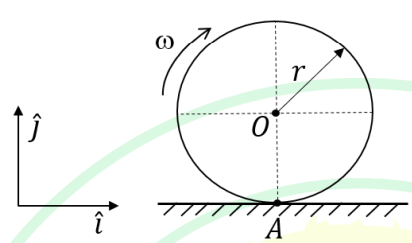
\includegraphics[width=0.5\columnwidth]{Figs/image (98).png}\caption*{}\label{fig:q26}\end{figure}
\vspace{0.2cm}
\begin{enumerate}
\begin{multicols}{2}
\item $r\omega\,\hat{i}$ and $0\,\hat{i}$
\item $g\omega\,\hat{i}$ and $0\,\hat{i}$
\item $r\omega\,\hat{i}$ and $g\omega\,\hat{i}$
\item $g\omega\,\hat{i}$ and $r\omega\,\hat{i}$
\end{multicols}
\end{enumerate}
\hfill{\brak{\text{GATE ME 2025}}}

\item
A truss structure is loaded as shown in the figure below. Among the options given, which member in the truss is a zero-force member?
\begin{figure}[H]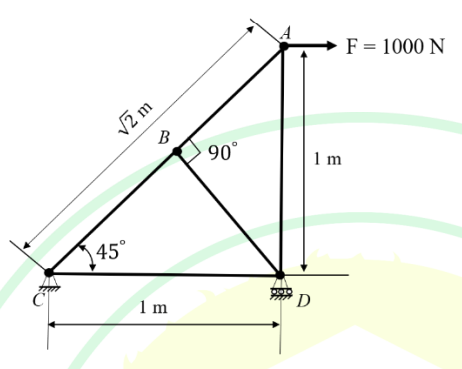
\includegraphics[width=0.5\columnwidth]{Figs/image (99).png}\caption*{}\label{fig:q27}\end{figure}
\vspace{0.2cm}
\begin{enumerate}
\begin{multicols}{2}
\item BD
\item BC
\item BA
\item AD
\end{multicols}
\end{enumerate}
\hfill{\brak{\text{GATE ME 2025}}}

\item
A metallic square plate is subjected to a uniform hydrostatic pressure $\brak{P}$. Choose the correct Mohr's circle representing the state of stress at any point in the plate from the options given below.\\
For the Mohr's circle, normal stress is positive towards right and shear stress is positive in the upward direction.

\vspace{0.2cm}
\begin{enumerate}
\begin{multicols}{2}
\item
\begin{figure}[H]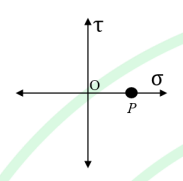
\includegraphics[width=0.5\columnwidth]{Figs/image (100).png}\caption*{}\label{fig:q28a}\end{figure}
\item
\begin{figure}[H]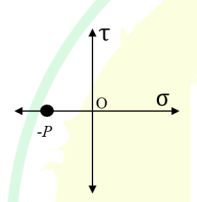
\includegraphics[width=0.5\columnwidth]{Figs/image - 2025-08-24T162257.117.png}\caption*{}\label{fig:q28a}\end{figure}
\item
\begin{figure}[H]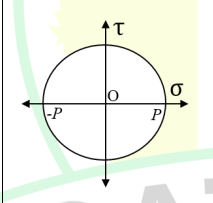
\includegraphics[width=0.5\columnwidth]{Figs/image - 2025-08-24T162356.507.png}\caption*{}\label{fig:q28a}\end{figure}
\item
\begin{figure}[H]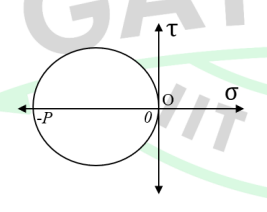
\includegraphics[width=0.5\columnwidth]{Figs/image - 2025-08-24T162433.675.png}\caption*{}\label{fig:q28a}\end{figure}
\end{multicols}
% (Omit figure since not provided; in real usage, include appropriate figure environment for options)
\end{enumerate}
\hfill{\brak{\text{GATE ME 2025}}}

\item
In the context of balancing of rotating and reciprocating masses, which one of the following options is true?

\vspace{0.2cm}
\begin{enumerate}
\begin{multicols}{2}
\item An unbalanced rigid rotor can be completely balanced using a single balancing mass
\item An unbalanced rigid rotor can be completely balanced using two balancing masses attached in two distinct planes
\item A single-cylinder internal combustion engine can be completely balanced using a single balancing mass
\item A single-cylinder internal combustion engine can be completely balanced using two balancing masses
\end{multicols}
\end{enumerate}
\hfill{\brak{\text{GATE ME 2025}}}

\item
A shaft carries a helical spur gear. Which one of the following bearings can NOT be used to support it?

\vspace{0.2cm}
\begin{enumerate}
\begin{multicols}{2}
\item Angular contact bearing
\item Double-row ball bearing
\item Straight roller bearing
\item Tapered roller bearing
\end{multicols}
\end{enumerate}
\hfill{\brak{\text{GATE ME 2025}}}



\item
The values of a function $f$ obtained for different values of $x$ are shown in the table below.

\begin{table}[ht]
\centering
\caption*{}
\label{tab:simpson}
\begin{tabular}{|c|c|c|c|c|c|}
\hline
$x$ & $0$ & $0.25$ & $0.5$ & $0.75$ & $1.0$ \\
\hline
$f(x)$ & $0.9$ & $2.0$ & $1.5$ & $1.8$ & $0.4$ \\
\hline
\end{tabular}
\end{table}

Using Simpson's one-third rule,\\
$\displaystyle \int_0^1 f(x) dx \approx$ \underline{\hspace{2cm}} \brak{\text{rounded off to 2 decimal places}}.

\hfill{\brak{\text{GATE ME 2025}}}

\item
The thermal efficiency of an ideal air-standard Otto cycle is $0.5$. The value of specific heat ratio of air is $1.4$. The compression ratio of the cycle is \underline{\hspace{2cm}} \brak{\text{rounded off to 1 decimal place}}.

\hfill{\brak{\text{GATE ME 2025}}}

\item
During a welding operation, thermal power of $2500$ W is incident normally on a metallic surface. As shown in the figure below \brak{\text{figure is NOT to scale}}, the heated area is circular. Out of the incident power, $85\%$ of the power is absorbed within a circle of radius $5$ mm while $65\%$ is absorbed within an inner concentric circle of radius $3$ mm. The power density in the shaded area is \underline{\hspace{2cm}} W mm$^{-2}$ \brak{\text{rounded off to 2 decimal places}}.
\begin{figure}[H]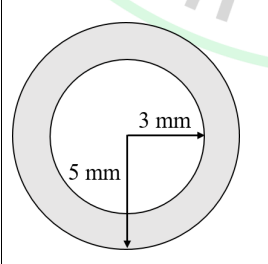
\includegraphics[width=0.5\columnwidth]{Figs/image - 2025-08-24T163425.703.png}\caption*{}\label{fig:q33}\end{figure}
\hfill{\brak{\text{GATE ME 2025}}}

\item
A liquid metal is poured in a mold cavity of size $200$ mm $\times$ $200$ mm $\times$ $200$ mm. The cooling is uniform in all directions with NO additional compensation for shrinkage. Considering the volumetric shrinkage during solidification and solid contraction as $7\%$ and $8\%$, respectively, the length of the cube edge after cooling down to the room temperature is \underline{\hspace{2cm}} mm \brak{\text{rounded off to 1 decimal place}}.

\hfill{\brak{\text{GATE ME 2025}}}

\item
A block of mass $1$ kg connected to a spring of stiffness $10$ N m$^{-1}$ is operating in a viscous medium such that the damping ratio $\brak{\text{or damping factor}}$ is equal to the ratio of the damped frequency to the natural frequency. The magnitude of the damping ratio for this system is \underline{\hspace{2cm}} \brak{\text{rounded off to 2 decimal places}}.

\hfill{\brak{\text{GATE ME 2025}}}

\item
In the closed interval $\brak{0,\, 3}$, the minimum value of the function $f$ given below is\\
$f(x) = 2x^3 - 9x^2 + 12x$\\
\begin{enumerate}
\begin{multicols}{2}
\item $0$
\item $4$
\item $5$
\item $9$
\end{multicols}
\end{enumerate}
\hfill{\brak{\text{GATE ME 2025}}}

\item
Considering the actual demand and the forecast for a product given in the table below, the mean forecast error and the mean absolute deviation, respectively, are

\begin{table}[ht]
\centering
\caption*{}
\label{tab:forecast}
\begin{tabular}{|c|c|c|c|c|c|c|c|c|c|c|}
\hline
Period & $1$ & $2$ & $3$ & $4$ & $5$ & $6$ & $7$ & $8$ & $9$ & $10$ \\
\hline
Actual demand & $425$ & $415$ & $420$ & $430$ & $427$ & $418$ & $422$ & $416$ & $426$ & $421$ \\
\hline
Forecast      & $427$ & $422$ & $416$ & $422$ & $423$ & $420$ & $419$ & $418$ & $430$ & $415$ \\
\hline
\end{tabular}
\end{table}

\begin{enumerate}
\begin{multicols}{2}
\item $0.8$ and $42.0$
\item $0.8$ and $4.2$
\item $8.0$ and $42.0$
\item $8.0$ and $4.2$
\end{multicols}
\end{enumerate}
\hfill{\brak{\text{GATE ME 2025}}}

\item
Match the mold elements in the casting process with the most suitable function
\begin{table}[ht]
\centering
\caption*{}
\label{tab:mold-match}
\begin{tabular}{|c|c|c|c|}
\hline
&Mold element & &Function\\
\hline
P &Blind riser & I& Casting with internal cavity\\
\hline
Q& Chill      & II& Molten metal reservoir\\
\hline
R& Skim bob  & III &Nucleating agent\\
\hline
S &Core      & IV &Assisting in faster heat removal from melt\\
\hline
T &Insulating sleeve & V& Removal of impurities\\
\hline
U& Inoculant  & VI& Increasing the solidification time\\
\hline
\end{tabular}
\end{table}
\begin{enumerate}
\begin{multicols}{2}
\item P-II, Q-IV, R-V, S-I, T-VI, U-III
\item P-II, Q-V, R-VI, S-I, T-III, U-IV
\item P-V, Q-I, R-VI, S-III, T-II, U-IV
\item P-II, Q-IV, R-I, S-V, T-VI, U-III
\end{multicols}
\end{enumerate}
\hfill{\brak{\text{GATE ME 2025}}}

\item
Wire drawing operation is performed on a perfectly plastic metal without any strain hardening. Assuming no friction and no redundant work, the maximum possible percentage reduction in area in a single pass is closest to
\begin{enumerate}
\begin{multicols}{2}
\item $51.2$
\item $63.2$
\item $75.0$
\item $93.2$
\end{multicols}
\end{enumerate}
\hfill{\brak{\text{GATE ME 2025}}}

\item
In relation to additive manufacturing, match the following


\begin{center}
\begin{tabularx}{\textwidth}{|c|X|X|}
\hline
\textbf{Process} & \textbf{Layer creation technique} & \textbf{Material} \\
\hline
P Stereolithography & 1 Injection of powder stream & I Paper \\
\hline
Q Fused deposition modeling & 2 Extrusion of melted polymer & II Epoxy \\
\hline
R Laminated object manufacturing & 3 Liquid layer curing & III Titanium \\
\hline
S Laser-engineered net shaping & 4 Sheet material deposition & IV Acrylonitrile butadiene styrene (ABS) \\
\hline
\end{tabularx}
\end{center}

\begin{enumerate}
\begin{multicols}{2}
\item P-$3$-III,\ Q-$1$-IV,\ R-$4$-I,\ S-$2$-II
\item P-$3$-II,\ Q-$2$-IV,\ R-$4$-I,\ S-$1$-III
\item P-$4$-III,\ Q-$2$-IV,\ R-$1$-II,\ S-$3$-I
\item P-$3$-II,\ Q-$2$-IV,\ R-$1$-I,\ S-$4$-III
\end{multicols}
\end{enumerate}
\hfill{\brak{\text{GATE ME 2025}}}

\item
A plate of $30\,\text{mm}$ thickness is fed through a rolling mill with two powered rolls. Each roll has a diameter of $500\,\text{mm}$. The plate thickness is to be reduced to $27\,\text{mm}$ in a single pass. Assume no change in width. The process feasibility and the maximum draft $\brak{\text{in mm}}$ can be represented, respectively, as\\
Use the coefficient of friction as $0.12$
\begin{enumerate}
\begin{multicols}{2}
\item feasible and $3.6$
\item NOT feasible and $2.6$
\item feasible and $3.0$
\item NOT feasible and $6.0$
\end{multicols}
\end{enumerate}
\hfill{\brak{\text{GATE ME 2025}}}

\item
The system shown in the figure below consists of a cantilever beam $\brak{\text{with flexural rigidity } EI \text{ and negligible mass}}$, a spring $\brak{\text{with spring constant } K \text{ and negligible mass}}$ and a block of mass $m$. Assuming a lumped parameter model for the system, the fundamental natural frequency $\brak{w_n}$ of the system is
\begin{figure}[H]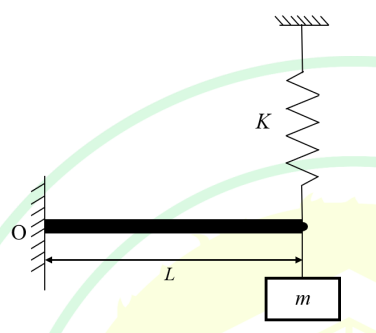
\includegraphics[width=0.5\columnwidth]{Figs/image - 2025-08-24T165339.288.png}\caption*{}\label{fig:q42}\end{figure}
\begin{enumerate}
\begin{multicols}{2}
\item $\sqrt{\dfrac{3EI}{L^3} + \dfrac{K}{m}}$
\item $\sqrt{\dfrac{EI}{L^3}+ K}$
\item $\sqrt{K/\left(3EI/L^3 + K\right)}$
\item $\sqrt{\dfrac{EI}{L^3}+ K/2m}$
\end{multicols}
\end{enumerate}
\hfill{\brak{\text{GATE ME 2025}}}

\item
The endurance limit of a specific grade of steel is same as its yield strength. The ultimate strength of this grade of steel is twice of its yield strength. A component made of this steel is loaded in tension and unloaded periodically. It is required that the component does NOT fail for at least $10^6$ loading cycles, as per the Soderberg law. Considering a factor of safety of $2$, the maximum applied tensile principal stress is
\begin{enumerate}
\begin{multicols}{2}
\item one-fourth of the endurance limit
\item half of the endurance limit
\item the endurance limit
\item twice the endurance limit
\end{multicols}
\end{enumerate}
\hfill{\brak{\text{GATE ME 2025}}}

\item
For a fully-developed pipe flow, which of the following options is/are correct?
\begin{enumerate}
\begin{multicols}{1}
\item For the same maximum velocity, the average velocity is higher in the turbulent regime than that of the laminar regime
\item Compressibility effects are important if Mach number is less than $0.3$
\item For laminar flow, the friction factor is independent of surface roughness
\item For laminar flow, friction factor decreases with decrease in Reynolds number
\end{multicols}
\end{enumerate}
\hfill{\brak{\text{GATE ME 2025}}}

\item
If $C$ is the unit circle in the complex plane with its center at the origin, then the value of $n$ in the equation given below is\\
$\displaystyle \int_C \dfrac{z^3}{\brak{z^2+4}\brak{z^2-4}}dz = 2\pi i n$\\
\underline{\hspace{2cm}} \brak{\text{rounded off to 1 decimal place}}.

\hfill{\brak{\text{GATE ME 2025}}}

\item
The directional derivative of the function $f$ given below at the point $(1,0)$ in the direction of $\dfrac{1}{2}\left(\hat{i}+ \sqrt{3}\hat{j}\right)$ is\\
$f(x,y) = x^2 + x y^2$\\
\underline{\hspace{2cm}} \brak{\text{rounded off to 1 decimal place}}.

\hfill{\brak{\text{GATE ME 2025}}}

\item
Let $y$ be the solution of the differential equation with the initial conditions given below. If $y\brak{x = 2} = A \ln 2$, then the value of $A$ is\\
$\dfrac{d^2y}{dx^2} + 3x + y= 0$,\quad $y\brak{x = 1} = 0$,\quad $\dfrac{dy}{dx}\brak{x = 1}=1$\\
\underline{\hspace{2cm}} \brak{\text{rounded off to 2 decimal places}}.

\hfill{\brak{\text{GATE ME 2025}}}

\item
Consider a cylindrical furnace of $5$ m diameter and $5$ m length with bottom, top and curved surfaces maintained at uniform temperatures of $800$ K, $1500$ K and $500$ K, respectively. The view factor between the bottom and top surfaces, $F_{12}$ is $0.2$. The magnitude of net radiation heat transfer rate between the bottom surface and the curved surface is \underline{\hspace{2cm}} kW \brak{\text{rounded off to 1 decimal place}}.\\
All surfaces of the furnace can be assumed as black.\\
The Stefan-Boltzmann constant, $\sigma = 5.67\times 10^{-8}\,\text{W}\,\text{m}^{-2}\,\text{K}^{-4}$.
\begin{figure}[H]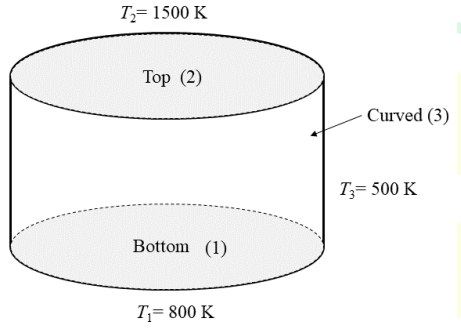
\includegraphics[width=0.5\columnwidth]{Figs/image - 2025-08-24T165555.549.png}\caption*{}\label{fig:q48}\end{figure}
\hfill{\brak{\text{GATE ME 2025}}}

\item
A pitot tube connected to a U-tube mercury manometer measures the speed of air flowing in the wind tunnel as shown in the figure below. The density of air is $1.23\,\text{kg}\,\text{m}^{-3}$ while the density of water is $1000\,\text{kg}\,\text{m}^{-3}$. For the manometer reading of $h = 30$ mm of mercury, the speed of air in the wind tunnel is\\
\underline{\hspace{2cm}} m s$^{-1}$ \brak{\text{rounded off to 1 decimal place}}.\\
Assume$\colon$ Specific gravity of mercury $=13.6$\\
Acceleration due to gravity $=10\,\text{m s}^{-2}$.
\begin{figure}[H]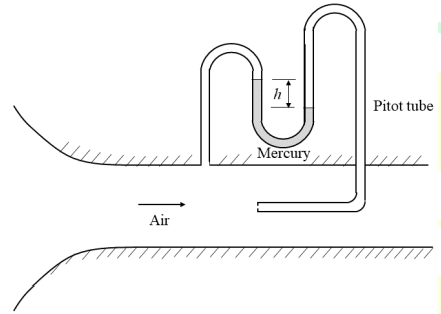
\includegraphics[width=0.5\columnwidth]{Figs/image - 2025-08-24T165912.948.png}\caption*{}\label{fig:q49}\end{figure}
\hfill{\brak{\text{GATE ME 2025}}}

\item
Consider a velocity field $v = 3z \hat{i} + 0 \hat{j} + Cx \hat{k}$, where $C$ is a constant. If the flow is irrotational, the value of $C$ is\\
\underline{\hspace{2cm}} \brak{\text{rounded off to 1 decimal place}}.

\hfill{\brak{\text{GATE ME 2025}}}

\item
Water enters a tube of diameter, $D = 60$ mm with mass flow rate of $0.01$ kg s$^{-1}$ as shown in the figure below. The inlet mean temperature is $T_{m,i} = 293$ K and the uniform heat flux at the surface of the tube is $2000$ W m$^{-2}$. For the exit mean temperature of $T_{m,o}= 353$ K, the length of the tube, $L$ is\\
\underline{\hspace{2cm}} m \brak{\text{rounded off to 1 decimal place}}.\\
Use the specific heat of water as $4181\,\text{J}\,\text{kg}^{-1}\,\text{K}^{-1}$.
\begin{figure}[H]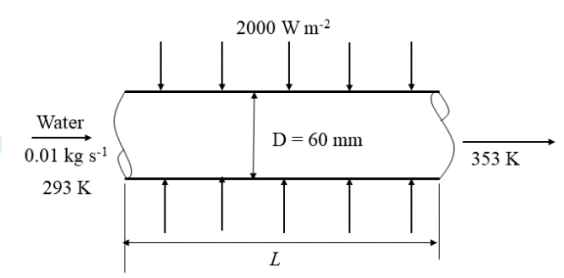
\includegraphics[width=0.5\columnwidth]{Figs/image - 2025-08-24T170258.389.png}\caption*{}\label{fig:q51}\end{figure}
\hfill{\brak{\text{GATE ME 2025}}}

\item
A thermal power plant is running with no reheat or regeneration. The specific enthalpy and specific entropy of steam at the turbine inlet are $3344\,\text{kJ}\,\text{kg}^{-1}$ and $6.5\,\text{kJ}\,\text{kg}^{-1}\,\text{K}^{-1}$, respectively. The turbine isentropic efficiency is $0.9$, and the mass flow rate of steam at the turbine inlet is $102\,\text{kg}\,\text{s}^{-1}$. The turbine power output is\\
\underline{\hspace{2cm}} MW \brak{\text{rounded off to 1 decimal place}}.

\begin{tabular}{|c|c|c|}
\hline
Properties & Saturated liquid water & Saturated water vapor\\
\hline
Specific enthalpy $\brak{\text{kJ kg}^{-1}}$ & $341$ & $2645$\\
\hline
Specific entropy $\brak{\text{kJ kg}^{-1}\,\text{K}^{-1}}$ & $1.1$ & $7.6$\\
\hline
\end{tabular}


\hfill{\brak{\text{GATE ME 2025}}}

\item
Consider a Pelton wheel of $1$ m diameter. The magnitude of relative velocity of water at the bucket inlet is same as the magnitude of relative velocity of water at the bucket exit. The absolute speed of water at the bucket inlet is $125.66$ m s$^{-1}$. For maximum power output from the Pelton wheel, the rpm of the Pelton wheel is\\
\underline{\hspace{2cm}} \brak{\text{rounded off to 1 decimal place}}.

\hfill{\brak{\text{GATE ME 2025}}}

\item
A thermodynamically closed system contains $1$ kg of hydrogen. The system undergoes a reversible polytropic process with polytropic index $1.3$. The work output during the process is $400$ kJ. During the process, hydrogen behaves as an ideal gas with constant specific heats. The absolute value of heat transfer during the process is\\
\underline{\hspace{2cm}} kJ \brak{\text{rounded off to 1 decimal place}}.\\
Specific heat of hydrogen at constant pressure $=14.56$ kJ kg$^{-1}$ K$^{-1}$\\
Specific heat of hydrogen at constant volume $=10.4$ kJ kg$^{-1}$ K$^{-1}$

\hfill{\brak{\text{GATE ME 2025}}}

\item
A heat pump, operating in reversed Carnot cycle, maintains a steady air temperature of $300$ K inside an auditorium. The heat pump receives heat from the ambient air. The ambient air temperature is $280$ K. Heat loss from the auditorium is $15$ kW. The power consumption of the heat pump is\\
\underline{\hspace{2cm}} kW \brak{\text{rounded off to 2 decimal places}}.

\hfill{\brak{\text{GATE ME 2025}}}

\item
The state of stress at a point is shown in the figure given below. Under plane stress assumption, the normal strain along the thickness direction $\brak{E_{zz}}$ is\\
\underline{\hspace{2cm}} \brak{\text{rounded off to 2 decimal places}}.\\
Use the Young's Modulus $E = 200$ GPa and Poisson's ratio $v = 0.27$.
\begin{figure}[H]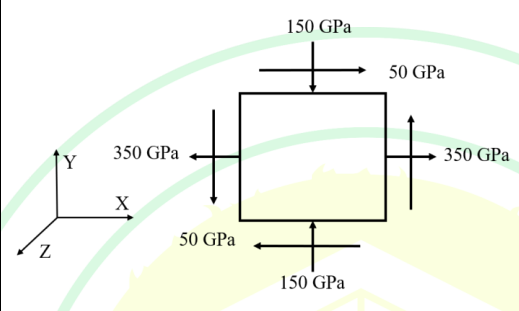
\includegraphics[width=0.5\columnwidth]{Figs/image - 2025-08-24T170617.692.png}\caption*{}\label{fig:q56}\end{figure}
\hfill{\brak{\text{GATE ME 2025}}}

\item
A simply supported beam of length $1$ m is subjected to a uniformly distributed bending moment of $1$ N m per m throughout the length as shown in the figure given below. The bending moment at the mid-point of the beam is\\
\underline{\hspace{2cm}} N m \brak{\text{rounded off to the nearest integer}}.
\begin{figure}[H]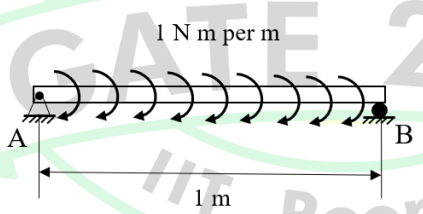
\includegraphics[width=0.5\columnwidth]{Figs/image - 2025-08-24T170702.548.png}\caption*{}\label{fig:q57}\end{figure}
\hfill{\brak{\text{GATE ME 2025}}}

\item
An isotropic brittle material is tested in the universal testing machine. The stress-strain diagram for the material shows a bi-linear elastic behavior as shown in the figure given below. The strain energy density is\\
\underline{\hspace{2cm}} MJ m$^{-3}$ \brak{\text{rounded off to 2 decimal places}}.
\begin{figure}[H]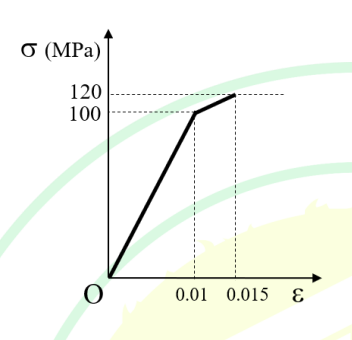
\includegraphics[width=0.5\columnwidth]{Figs/image - 2025-08-24T170750.530.png}\caption*{}\label{fig:q58}\end{figure}
\hfill{\brak{\text{GATE ME 2025}}}

\item
A pair of spur gears is required to maintain a velocity ratio of $1\colon 2$. The module of the gears is $10$ mm and the addendum is $10$ mm. If the operating pressure angle is $15\degree$, the minimum number of teeth required on the pinion to ensure NO interference/undercutting is\\
\underline{\hspace{2cm}} \brak{\text{answer in integer}}.

\hfill{\brak{\text{GATE ME 2025}}}

\item
An offset slider-crank mechanism is shown in the figure below. The length of the stroke of the slider is\\
\underline{\hspace{2cm}} mm \brak{\text{rounded off to nearest integer}}.
\begin{figure}[H]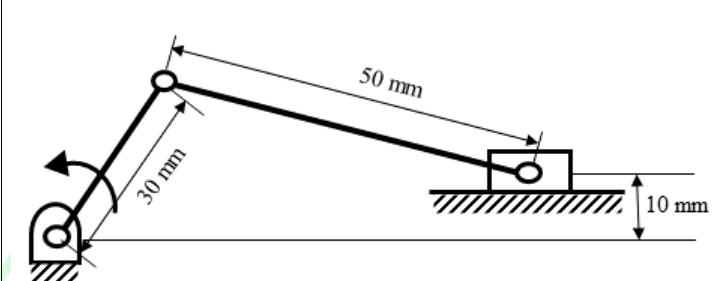
\includegraphics[width=0.5\columnwidth]{Figs/image - 2025-08-24T170849.218.png}\caption*{}\label{fig:q60}\end{figure}
\hfill{\brak{\text{GATE ME 2025}}}

\item
Two plates of thickness $10$ mm each are to be joined by a transverse fillet weld on one side and the resulting structure is loaded as shown in the figure below. If the ultimate tensile strength of the weld material is $150$ MPa and the factor of safety to be used is $3$, the minimum length of the weld required to ensure that the weld does NOT fail is\\
\underline{\hspace{2cm}} mm \brak{\text{rounded off to 2 decimal places}}.
\begin{figure}[H]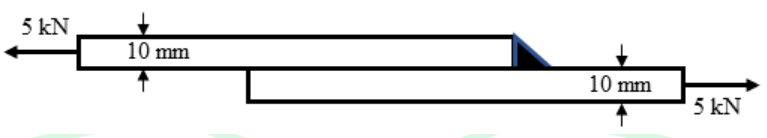
\includegraphics[width=0.5\columnwidth]{Figs/image - 2025-08-24T170927.609.png}\caption*{}\label{fig:q61}\end{figure}
\hfill{\brak{\text{GATE ME 2025}}}

\item
Two metal parts (a cylinder and a cube) of same volume are cast under identical conditions. The diameter of the cylinder is equal to its height. The ratio of the solidification time of the cube to that of the cylinder is\\
\underline{\hspace{2cm}} \brak{\text{rounded off to 2 decimal places}}.\\
Assume that solidification time follows Chvorinov's rule with an exponent of $2$.

\hfill{\brak{\text{GATE ME 2025}}}

\item
Cylindrical workpieces of diameter $60$ mm and length $400$ mm are machined on a lathe at a cutting speed of $25$ m min$^{-1}$ and a feed of $0.2$ mm rev$^{-1}$. The Taylor's tool life parameters $C$ and $n$ for this setup are $75$ and $0.25$, respectively. The tool changing time is $3$ minutes. With a labor and overhead cost of $5$ per minute, the tool changing cost per piece is\\
\underline{\hspace{2cm}} \brak{\text{rounded off to 2 decimal places}}.

\hfill{\brak{\text{GATE ME 2025}}}

\item
A company uses $3000$ units of a part annually. The units are priced as given in the table below. It costs  Rs $150$ to place an order. Carrying costs are $40$ percent of the purchase price per unit on an annual basis. The minimum total annual cost is\\
\underline{\hspace{2cm}} \brak{\text{rounded off to 1 decimal place}}.

\begin{table}[ht]
\centering
\caption*{}
\label{tab:annual-cost}
\begin{tabular}{|c|c|}
\hline
Order quantity & Unit price\\
\hline
$1$ to $499$ & $9.0$\\
\hline
$500$ to $999$ & $8.5$\\
\hline
$1000$ or more & $8.0$\\
\hline
\end{tabular}
\end{table}

\hfill{\brak{\text{GATE ME 2025}}}

\item
A project involves eight activities with the precedence relationship and duration as shown in the table below. The slack for the activity D is \underline{\hspace{2cm}} hours \brak{\text{answer in integer}}.


\begin{tabular}{|c|c|c|}
\hline
Activity & Immediate predecessor & Duration \brak{\text{hours}}\\
\hline
A & - & $4$\\
\hline
B & A & $8$\\
\hline
C & A & $5$\\
\hline
D & B & $2$\\
\hline
E & B & $7$\\
\hline
F & C & $6$\\
\hline
G & D & $3$\\
\hline
H & E, F, G & $9$\\
\hline
\end{tabular}


\hfill{\brak{\text{GATE ME 2025}}}
\end{enumerate}




\end{document}